%%%%%%%%%%%%%%%%%%%%%%%%%%%%%%%%%%%%%%%%%
% Beamer Presentation
% LaTeX Template
% Version 1.0 (10/11/12)
%
% This template has been downloaded from:
% http://www.LaTeXTemplates.com
%
% License:
% CC BY-NC-SA 3.0 (http://creativecommons.org/licenses/by-nc-sa/3.0/)
%
%%%%%%%%%%%%%%%%%%%%%%%%%%%%%%%%%%%%%%%%%

%----------------------------------------------------------------------------------------
%	PACKAGES AND THEMES
%----------------------------------------------------------------------------------------

\documentclass{beamer}

\mode<presentation> {

% The Beamer class comes with a number of default slide themes
% which change the colors and layouts of slides. Below this is a list
% of all the themes, uncomment each in turn to see what they look like.

%\usetheme{default}
%\usetheme{AnnArbor}
%\usetheme{Antibes}
%\usetheme{Bergen}
%\usetheme{Berkeley}
%\usetheme{Berlin}
%\usetheme{Boadilla}
%\usetheme{CambridgeUS}
%\usetheme{Copenhagen}
%\usetheme{Darmstadt}
%\usetheme{Dresden}
%\usetheme{Frankfurt}
%\usetheme{Goettingen}
%\usetheme{Hannover}
%\usetheme{Ilmenau}
%\usetheme{JuanLesPins}
%\usetheme{Luebeck}
\usetheme{Madrid}
%\usetheme{Malmoe}
%\usetheme{Marburg}
%\usetheme{Montpellier}
%\usetheme{PaloAlto}
%\usetheme{Pittsburgh}
%\usetheme{Rochester}
%\usetheme{Singapore}
%\usetheme{Szeged}
%\usetheme{Warsaw}

% As well as themes, the Beamer class has a number of color themes
% for any slide theme. Uncomment each of these in turn to see how it
% changes the colors of your current slide theme.

%\usecolortheme{albatross}
%\usecolortheme{beaver}
%\usecolortheme{beetle}
%\usecolortheme{crane}
%\usecolortheme{dolphin}
%\usecolortheme{dove}
%\usecolortheme{fly}
%\usecolortheme{lily}
%\usecolortheme{orchid}
%\usecolortheme{rose}
%\usecolortheme{seagull}
%\usecolortheme{seahorse}
%\usecolortheme{whale}
%\usecolortheme{wolverine}

%\setbeamertemplate{footline} % To remove the footer line in all slides uncomment this line
%\setbeamertemplate{footline}[page number] % To replace the footer line in all slides with a simple slide count uncomment this line

%\setbeamertemplate{navigation symbols}{} % To remove the navigation symbols from the bottom of all slides uncomment this line
}

\usepackage{graphicx} % Allows including images
\usepackage{booktabs} % Allows the use of \toprule, \midrule and \bottomrule in tables
\usepackage{multirow}
\usepackage{adjustbox}
\usepackage{array}
\usepackage{tikz}
\usetikzlibrary{shapes.geometric, arrows, positioning, fit}
\usepackage[latin1]{inputenc}
\newcommand{\xmark}{\textcolor{red}{\text{\sffamily X}}}
\newcommand{\cmark}{\textcolor{green}{\checkmark}}
\newcommand{\tr}{\text{tr}}
\newcommand{\E}{\textbf{E}}
\newcommand{\diag}{\text{diag}}
\newcommand{\argmax}{\text{argmax}}
\newcommand{\argmin}{\text{argmin}}
\newcommand{\Cov}{\text{Cov}}
\newcommand{\Vol}{\text{Vol}}
\newcommand{\bx}{\boldsymbol{x}}
\newcommand{\by}{\boldsymbol{y}}
\newcommand{\bX}{\boldsymbol{X}}
\newcommand{\bY}{\boldsymbol{Y}}

%tikz stufff


%----------------------------------------------------------------------------------------
%	TITLE PAGE
%----------------------------------------------------------------------------------------


\title[Informal]{How many neurons does it take to classify a lightbulb?}

\author{Charles Zheng} % Your name
\institute[Stanford] % Your institution as it will appear on the bottom of every slide, may be shorthand to save space
{Stanford University}
\date{\today} % Date, can be changed to a custom date

\begin{document}

\begin{frame}
\titlepage % Print the title page as the first slide
(Joint work with Yuval Benjamini)
\end{frame}

\begin{frame}
\frametitle{Overview}
\noindent\emph{Background and motivation}
\begin{itemize}
\item Review of information theory
\item Study of neural coding
\end{itemize}
\noindent\emph{Problems}
\begin{itemize}
\item Estimating mutual information between stimulus and response.
\item Can we use machine learning methods to estimate MI?
\end{itemize}
\noindent\emph{Methods}
\begin{itemize}
\item Setup
\item Gaussian example
\item Using Fano's inequality
\item Using low-SNR universality
\end{itemize}
\noindent\emph{Results}
\end{frame}

\section{Background}


\begin{frame}
\frametitle{Information theory} 
The complexity of modern communications system is made possible by Shannon's theory of information.
\vspace{0.4in}
\begin{center}
\begin{tabular}{cc}
\includegraphics[scale =0.3]{communication-entry.png} &
\includegraphics[scale =  0.2]{relay_channel.jpg}
\end{tabular}
\end{center}
\vspace{0.4in}
A information-processing network can be analyzed in terms of interactions between its components (which are viewed as random variables.)

\tiny{Image credit CartouCHe, Aziz et al. 2011}
\note{ Modern communication systems depend
  on a vast network of signal transmitters and receivers.  All of this
  sophisticated engineering is made possible by information theory, a
  branch of applied mathematics introduced by Claude Shannon in 1948.
  Under the lens of information theory, we decompose a information
  network (e.g. the internet) into individual components (e.g. a
  server, a satellite) and view this collection of components as a
  collection of random variables, similar to a probabilistic graphical
  model.  Information theory defines quantities such as entropy,
  conditional entropy, and mutual information which serve to quantify
  how much information is contained in each component, and how the
  information is transmitted or lost as it passes through the network.
}
\end{frame}

\begin{frame}
\frametitle{Entropy and mutual information}
$X$ and $Y$ have joint density $p(x, y)$ with respect to $\mu$.

\vspace{0.5in}

\begin{tabular}{c|c|c}
\hline
Quantity & Definition & Linear analogue\\\hline
Entropy & $H(X) = - \int (\log p(x)) p(x) \mu_X(dx)$ & $\text{Var}(X)$\\
Conditional entropy & $H(X|Y) = \E[H(X|Y)]$ & $\E[\text{Var}(X|Y)]$\\
Mutual information & $I(X;Y) = H(X) - H(X|Y)$ & $\text{Cor}(X, Y)$\\\hline
\end{tabular}

\vspace{0.3in}

\small{The above definition includes both \emph{differential} entropy and \emph{discrete} entropy.
Information theorists tend to use log base 2, we will use natural logs in this talk.}
\end{frame}

\begin{frame}
\frametitle{Properties of mutual information}
\begin{center}
\includegraphics[scale = 0.2]{kinney.png}
\end{center}
\begin{itemize}
\item Nonnegative: $I(X;Y) \geq 0$
\item Symmetric: $I(X;Y) = I(Y; X)$
\item Bijection-invariant: $I(\phi(X); \psi(Y)) = I(\psi(Y);\phi(X)$.
\item Additivity.  If $(X_1,Y_1) \perp (X_2, Y_2)$, then
\[
I((X_1, X_2); (Y_1, Y2)) = I(X_1; Y_1) + I(X_2; Y_2)
\]
\item Relation to KL divergence $\mathbb{D}$.
\[
\mathbb{D}(p(x, y)||p(x)p(y)) = I(X; Y)
\]
\end{itemize}
\tiny{Image credit Kinney et al. 2014}
\end{frame}

\begin{frame}
\frametitle{Studying the neural code}
The brain is the \emph{most complex} information processing system we know!
\vspace{0.3in}
\begin{center}
\begin{tabular}{cc}
\includegraphics[scale = 0.3, clip =true, trim=0 0 0 2.5in]{Brain_network.png} &
\includegraphics[scale = 0.1]{maxresdefault.jpg}\\
\small{Neural network inferred from data} & \small{Organization of human retina}\\
\small{(Hong et al.)} & 
\end{tabular}
\end{center}
\vspace{0.3in}
How do neurons encode, process, and decode sensory information?

\tiny{Image credit: Hong et al., Interactive Biology}
\end{frame}


\begin{frame}
\frametitle{Studying the neural code: data}
\begin{center}
\includegraphics[scale = 0.2]{quiroga.png}
\end{center}
\begin{itemize}
\item  Let $\mathcal{X}$ define a class of stimuli (faces, objects, sounds.)
\item Stimulus $\bX = (X_1,\hdots, X_p)$, where $X_i$ are features (e.g. pixels.)
\item Present $\bX$ to the subject, record the subject's brain activity using EEG, MEG, fMRI, or calcium imaging.
\item Recorded response $\bY = (Y_1,\hdots, Y_q)$, where $Y_i$ are single-cell responses, or recorded activities in different brain region. 
\end{itemize}
\tiny{Image credits: Quiroga et al. (2009)}
\end{frame}


\section{Problems}

\begin{frame}
\frametitle{Problem statement}
Given stimulus-reponse data $(\bX, \bY)$, can we estimate the mutual information $I(\bX; \bY)$?

\vspace{0.5in}
\emph{Why do we care?}
\begin{itemize}
\item Selecting the correct model for neural encoding
\item Assessing the \emph{efficiency} of the neural code
\item Measuring the \emph{redundancy} of a population of neurons
\[
r' = \frac{\sum_{i=1}^q I(\bX; Y_i) - I(\bX; \bY)}{\sum_{i=1}^q I(\bX; Y_i)}
\]
\end{itemize}
\end{frame}


\begin{frame}
\frametitle{Experimental setup}
\begin{itemize}
\item How to make inferences about the population of stimuli in
  $\mathcal{X}$ using finitely many examples?
\item \emph{Randomization.}  Select $\bX^{(1)},\hdots,
  \bX^{(K)}$ randomly from some distribution $p(\bx)$ (e.g. an image
  database).  Record $r$ responses from each stimulus.
\end{itemize}
\begin{center}
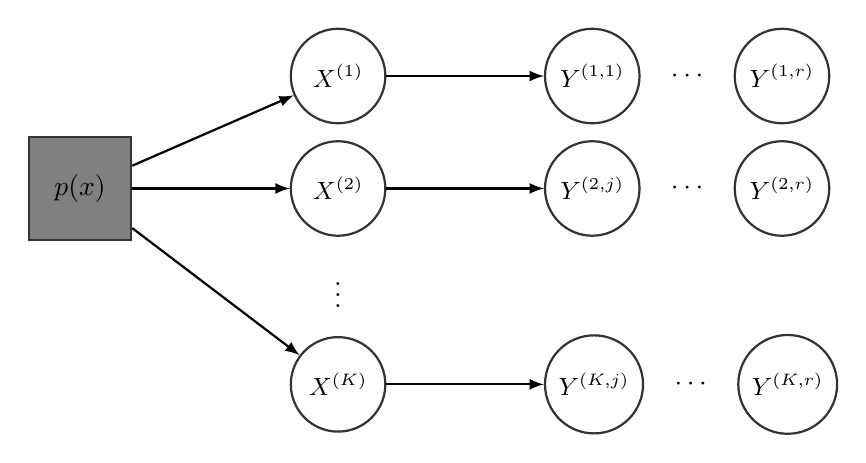
\begin{tikzpicture}[node distance = 2mm and 20mm]
\tikzstyle{main} = [circle, minimum size = 12mm, thick, draw = black!80]
\tikzstyle{main0} = [circle, minimum size = 2mm, thick, draw = white!100]
\tikzstyle{param} = [rectangle, minimum size = 13mm, thick, draw = black!80]
\tikzstyle{connect} = [-latex, thick]
\tikzstyle{box} = [rectangle, draw = black!100]
  \node[param, fill = black!50] (px) {$p(\bx)$};
  \node[main, right=of px] (x2) {\small{$\bX^{(2)}$}};
  \node[main, above=of x2] (x1) {\small{$\bX^{(1)}$}};
  \node[main0, below=of x2] (xdots) {$\vdots$};
  \node[main, below=of xdots] (x3) {\small{$\bX^{(K)}$}};
  \node[main, right=of x1] (y11) {\small{$\bY^{(1,1)}$}};
  \node[main, right=of x2] (y21) {\small{$\bY^{(2,j)}$}};
  \node[main, right=of x3] (y31) {\small{$\bY^{(K,j)}$}};
\begin{scope}[node distance = 3mm and 2mm]
  \node[main0, right=of y11] (y12) {$\cdots$};
  \node[main0, right=of y21] (y22) {$\cdots$};
  \node[main0, right=of y31] (y32) {$\cdots$};
  \node[main, right=of y12] (y13) {\small{$\bY^{(1,r)}$}};
  \node[main, right=of y22] (y23) {\small{$\bY^{(2,r)}$}};
  \node[main, right=of y32] (y33) {\small{$\bY^{(K,r)}$}};
\end{scope}
\path (px) edge [connect] (x1) (px) edge [connect] (x2) (px) edge [connect] (x3)
      (x1) edge [connect] (y11) (x2) edge [connect] (y21) (x3) edge [connect] (y31);
\end{tikzpicture}
\end{center}
\end{frame}

\begin{frame}
\frametitle{Can we learn $I(\bX; \bY)$ from such data?}
Answer: yes.
\begin{itemize}
\item Let $p^*(\bx)$ be the uniform distribution over $\bX^{(1)}, \hdots, \bX^{(K)}$, and let $\tilde{\bX}$ be a random vector with this distribution.
\item Let $\tilde{\bY}$ have the distribution
\[
p^*(\tilde{\by}) = \frac{1}{K} \sum_{i=1}^K p(\by|\bx^{(i)})
\] 
\item Then, as $K \to \infty$,  $I(\tilde{\bX}; \tilde{\bY})  \stackrel{p}{\to} I(\bX; \bY)$, where
\[
I(\tilde{\bX}; \tilde{\bY}) = H(\tilde{\bY}) - \frac{1}{K}\sum_{i=1}^K H(\bY| \bX^{(i)})
\]
\item We can apply nonparametric methods to estimate
  $H(\bY|\bX^{(i)})$ for $i = 1,\hdots, K$, and
  $H(\tilde{\bY})$. Plugging those estimates into the above formula
  gives a \emph{nonparametric} estimate of $I(\bX; \bY)$.
\end{itemize}
\end{frame}

\begin{frame}
\frametitle{References}
\begin{itemize}
\item Cover and Thomas.  Elements of information theory.
\item Muirhead.  Aspects of multivariate statistical theory.
\item van der Vaart.  Asymptotic statistics.
\end{itemize}
\end{frame}

\end{document}




\begin{itemize}
\item 
\item Define a distribution $p(\bx)$ supported on $\mathcal{X}$.  \emph{In practice, $p(\bx)$ may be represented as a large image database.}
\item Sample stimuli $\bX^{(1)}, \hdots, \bX^{(K)}$ from $p(x)$. \emph{I.e., draw $K$ images from the image database.}
\item For $i = 1,\hdots, K$, present the subject with stimulus
  $\bX^{(1)}$, record the neural response $\bY^{(i, j)}$.  For each
  stimulus, obtain repeats $j = 1,\hdots, r$.
\end{itemize}








